\documentclass[12pt,a4paper]{article}

\usepackage[utf8]{inputenc}
\usepackage[T1]{fontenc}
\usepackage[brazil]{babel}
\usepackage{indentfirst}

\usepackage[top=3cm,bottom=2cm,left=3cm,right=2cm]{geometry}
\usepackage{setspace}
\onehalfspacing
\usepackage{mathptmx}          


\usepackage{graphicx}
\usepackage{booktabs}
\usepackage{multirow}
\usepackage{float}
\usepackage{caption}
\usepackage{amsmath,amssymb}
\usepackage{listings}
\usepackage{xcolor}
\usepackage[hidelinks]{hyperref}


\captionsetup{font=small,labelsep=endash,justification=centering}
\captionsetup[table]{position=top}
\captionsetup[figure]{position=top}


\newcommand{\fonte}[1]{%
  \vspace{-2mm}
  \begin{center}\footnotesize Fonte: #1\end{center}
}


\lstdefinestyle{python}{
  language=Python,
  basicstyle=\ttfamily\footnotesize,
  keywordstyle=\color{blue},
  commentstyle=\color{gray},
  stringstyle=\color{teal},
  numbers=left, numberstyle=\tiny, numbersep=8pt,
  breaklines=true, frame=single, showstringspaces=false
}

\begin{document}


\begin{titlepage}
\begin{center}


\includegraphics[width=0.65\textwidth]{../figuras/logo-unifor.png}\\[0.5cm]


{\large CENTRO DE CIÊNCIAS TECNOLÓGICAS -- CCT}\\[0.3cm]
{\large Métodos Quantitativos em Computação}\\[0.2cm]
{\normalsize Professor Cledinaldo Castro Araújo}

\vfill

{\Huge \textbf{Relatório Descritivo}}\\[0.6cm]
{\Large Análise dos Crimes Violentos Letais Intencionais (CVLI)\\ no Estado do Ceará --- 2009 a 2025}

\vfill

{\large \textbf{Alunos:}}\\[0.2cm]
{\large Matheus Cruz --- Matrícula: 2517389}\\[0.1cm]
{\large Guilherme Azevedo --- Matrícula: 2510423}\\[0.1cm]
{\large Samuel Lopes --- Matrícula: 2510371}\\[0.1cm]
{\large Enzo Fernandes --- Matrícula: 2510425}\\[0.1cm]
{\large Rodrigo Temporal --- Matrícula: 2510402}

\vfill

{\large Fortaleza, Setembro de 2026}

\end{center}
\end{titlepage}


\renewcommand{\contentsname}{Sumário}
\tableofcontents
\newpage


\section{Introdução}

A violência letal constitui um dos principais desafios de segurança pública no Brasil. No Ceará, os Crimes Violentos Letais Intencionais (CVLI) reúnem os registros de homicídio doloso, feminicídio, lesão corporal seguida de morte e latrocínio, sendo o indicador oficial utilizado pela Secretaria da Segurança Pública e Defesa Social (SSPDS) para o monitoramento da criminalidade violenta no estado.

A análise descritiva de dados assume papel central nesse cenário, pois permite organizar grandes volumes de registros, revelar padrões temporais e de perfil das vítimas, e subsidiar decisões estratégicas de alocação de efetivo policial, formulação de políticas de prevenção à violência e direcionamento de investimentos em segurança pública. Por meio de distribuições de frequência, tabelas cruzadas, gráficos e medidas resumo, é possível transformar dados brutos em informação acessível e fundamentada, contribuindo para uma tomada de decisão baseada em evidências.

Diante disso, este relatório apresenta uma análise descritiva da base de CVLI do Estado do Ceará entre 2009 e 2025, totalizando 59.340 registros. O estudo está organizado em séries estatísticas (distribuições de frequência por natureza do crime, meio empregado, gênero, escolaridade, raça e dia da semana), tabelas cruzadas (meio empregado $\times$ gênero; escolaridade $\times$ raça), representações gráficas (setores, barras, linhas e boxplot) e medidas de posição e dispersão aplicadas à variável idade da vítima.

\newpage


\section{Objetivos}

\subsection{Objetivo Geral}

Fornecer subsídios descritivos para a análise dos Crimes Violentos Letais Intencionais (CVLI) no Estado do Ceará, no período de 2009 a 2025.

\subsection{Objetivos Específicos}

\begin{itemize}
    \item Descrever a ocorrência dos Crimes Violentos Letais Intencionais (CVLI) no Estado do Ceará, considerando sua distribuição temporal e espacial;
    \item Organizar e apresentar indicadores descritivos, por meio de tabelas, gráficos e medidas estatísticas, que permitam a compreensão do cenário da violência letal no estado;
    \item Identificar o perfil predominante das vítimas de CVLI quanto a gênero, faixa etária, escolaridade e raça/cor, bem como os meios empregados e os períodos de maior incidência.
\end{itemize}

\newpage


\section{Metodologia}

\subsection{Natureza e fonte dos dados}

Trata-se de um estudo de natureza quantitativa, descritiva, com dados secundários. Os dados foram obtidos junto à Secretaria da Segurança Pública e Defesa Social do Estado do Ceará (SSPDS/CE), por meio dos indicadores detalhados disponibilizados publicamente no portal do Governo do Estado, referentes ao período de 2009 a 2025.

\subsection{Amostra}

A base analisada é composta por 59.340 registros de CVLI. Após o tratamento, foram considerados 59.340 registros válidos, com conversão de campos numéricos (idade) para formato adequado e descarte de valores ausentes apenas nas análises específicas da variável idade (54.206 registros válidos de idade).

\subsection{Ferramentas computacionais}

O tratamento e a análise dos dados foram realizados na linguagem \textbf{Python} (versão 3.12), utilizando as bibliotecas \texttt{pandas} (manipulação e agregação), \texttt{numpy} (cálculos estatísticos) e \texttt{matplotlib} (visualização). O ambiente de execução foi o terminal local com script dedicado. A rotina computacional utilizada encontra-se no Apêndice~\ref{ap:codigo}.

\subsection{Classificação das variáveis}

\begin{table}[H]
\centering
\caption{Classificação das variáveis analisadas}
\label{tab:variaveis}
\begin{tabular}{lll}
\toprule
\textbf{Variável} & \textbf{Tipo} & \textbf{Nível de mensuração} \\
\midrule
Natureza               & Qualitativa  & Nominal   \\
Meio empregado         & Qualitativa  & Nominal   \\
Gênero da vítima       & Qualitativa  & Nominal   \\
Escolaridade da vítima & Qualitativa  & Ordinal   \\
Raça da vítima         & Qualitativa  & Nominal   \\
Dia da semana          & Qualitativa  & Ordinal   \\
Idade da vítima        & Quantitativa & Contínua (razão) \\
Data (mês/ano)         & Quantitativa & Intervalar \\
Hora                   & Quantitativa & Intervalar \\
\bottomrule
\end{tabular}
\end{table}
\fonte{Elaborada pelos autores (2026).}

Entende-se, a partir da Tabela~\ref{tab:variaveis}, que predominam variáveis qualitativas nominais (natureza, meio empregado, gênero e raça), o que justifica o uso de distribuições de frequência simples e relativa como principal recurso descritivo. As variáveis ordinais (escolaridade e dia da semana) permitem ordenação natural, enquanto a variável quantitativa contínua (idade) possibilita o cálculo de medidas de posição e dispersão.

\subsection{Cronograma}

\begin{table}[H]
\centering
\caption{Cronograma de execução da atividade}
\label{tab:cronograma}
\begin{tabular}{lll}
\toprule
\textbf{Etapa} & \textbf{Descrição} & \textbf{Período} \\
\midrule
1 & Coleta e organização dos dados & 01/09 a 02/09 \\
2 & Tratamento e limpeza da base   & 02/09 a 03/09 \\
3 & Análise descritiva em Python   & 03/09 a 05/09 \\
4 & Elaboração do relatório        & 05/09 a 07/09 \\
5 & Revisão e apresentação oral    & 07/09 a 08/09 \\
\bottomrule
\end{tabular}
\end{table}
\fonte{Elaborada pelos autores (2026).}

\newpage


\section{Análise e Interpretação dos Dados}

\subsection{Séries estatísticas}

\subsubsection{Natureza}

\begin{table}[H]
\centering
\caption{Distribuição dos CVLI segundo a natureza do crime, Ceará, 2009--2025}
\label{tab:natureza}
\begin{tabular}{lrr}
\toprule
\textbf{Natureza} & \textbf{Frequência simples (f)} & \textbf{Frequência relativa (\%)} \\
\midrule
Homicídio doloso                  & 57.367 & 96,68 \\
Latrocínio                        & 1.003  & 1,69  \\
Lesão corporal seguida de morte   & 689    & 1,16  \\
Feminicídio                       & 281    & 0,47  \\
\midrule
\textbf{Total}                    & \textbf{59.340} & \textbf{100,0} \\
\bottomrule
\end{tabular}
\end{table}
\fonte{SSPDS/CE (2026). Elaborada pelos autores.}

Conclui-se, com base na Tabela~\ref{tab:natureza}, que o homicídio doloso é amplamente predominante, respondendo por 96,68\% de todos os registros de CVLI no período analisado. Latrocínio (1,69\%) e lesão corporal seguida de morte (1,16\%) aparecem como categorias secundárias, enquanto o feminicídio representa apenas 0,47\% dos registros --- percentual que pode refletir tanto a menor incidência proporcional quanto a subnotificação histórica dessa tipificação, que só foi incluída no Código Penal brasileiro em 2015 (Lei n.º 13.104/2015).


\subsubsection{Meio empregado}

\begin{table}[H]
\centering
\caption{Distribuição dos CVLI segundo o meio empregado, Ceará, 2009--2025}
\label{tab:meio}
\begin{tabular}{lrr}
\toprule
\textbf{Meio empregado} & \textbf{f} & \textbf{\%} \\
\midrule
Arma de fogo    & 49.573 & 83,54 \\
Arma branca     & 6.071  & 10,23 \\
Outros meios    & 3.355  & 5,65  \\
Não informado   & 341    & 0,57  \\
\midrule
\textbf{Total}  & \textbf{59.340} & \textbf{100,0} \\
\bottomrule
\end{tabular}
\end{table}
\fonte{SSPDS/CE (2026). Elaborada pelos autores.}

Entende-se, pela Tabela~\ref{tab:meio}, que a arma de fogo é o meio empregado em mais de 83\% dos crimes violentos letais no Ceará, confirmando a forte associação entre a disponibilidade de armas de fogo ilegais e a letalidade criminal no estado. A arma branca aparece em 10,23\% dos casos, indicando que, mesmo em menor proporção, instrumentos cortantes e perfurantes também constituem um meio relevante de agressão letal. O baixo percentual de ``não informado'' (0,57\%) sugere boa qualidade no registro dessa variável pela SSPDS.


\subsubsection{Gênero da vítima}

\begin{table}[H]
\centering
\caption{Distribuição das vítimas de CVLI segundo o gênero, Ceará, 2009--2025}
\label{tab:genero}
\begin{tabular}{lrr}
\toprule
\textbf{Gênero} & \textbf{f} & \textbf{\%} \\
\midrule
Masculino      & 54.748 & 92,26 \\
Feminino       & 4.575  & 7,71  \\
Não identificado  & 17     & 0,03  \\
\midrule
\textbf{Total} & \textbf{59.340} & \textbf{100,0} \\
\bottomrule
\end{tabular}
\end{table}
\fonte{SSPDS/CE (2026). Elaborada pelos autores.}

Observa-se, na Tabela~\ref{tab:genero}, que homens constituem a esmagadora maioria das vítimas de CVLI no Ceará, representando 92,26\% do total. Esse padrão é consistente com a literatura criminológica nacional, que aponta homens jovens como o grupo mais vulnerável à violência letal, tanto pela maior exposição a situações de risco (conflitos interpessoais, envolvimento com o tráfico de drogas) quanto por fatores socioculturais associados à masculinidade e à resolução violenta de conflitos.

\subsubsection{Escolaridade da vítima}

\begin{table}[H]
\centering
\caption{Distribuição das vítimas de CVLI segundo a escolaridade, Ceará, 2009--2025}
\label{tab:escolaridade}
\begin{tabular}{lrr}
\toprule
\textbf{Escolaridade} & \textbf{f} & \textbf{\%} \\
\midrule
Não Alfabetizado                 & 2.239  & 3,77  \\
Alfabetizado                     & 16.798 & 28,31 \\
Ensino Fundamental Incompleto    & 9.379  & 15,81 \\
Ensino Fundamental Completo      & 6.458  & 10,88 \\
Ensino Médio Incompleto          & 2.620  & 4,42  \\
Ensino Médio Completo            & 4.457  & 7,51  \\
Superior Incompleto              & 240    & 0,40  \\
Superior Completo                & 273    & 0,46  \\
Não Informada                    & 16.876 & 28,44 \\
\midrule
\textbf{Total}               & \textbf{59.340} & \textbf{100,0} \\
\bottomrule
\end{tabular}
\end{table}
\fonte{SSPDS/CE (2026). Elaborada pelos autores.}

Conclui-se, a partir da Tabela~\ref{tab:escolaridade}, que as vítimas de CVLI concentram-se majoritariamente nos níveis mais baixos de escolaridade. Somando-se as categorias ``Alfabetizado'' (28,31\%) e ``Ensino Fundamental Incompleto'' (15,81\%), tem-se que mais de 44\% das vítimas com escolaridade informada possuem, no máximo, o ensino fundamental incompleto. Vítimas com ensino superior (completo ou incompleto) representam menos de 1\% do total. O alto percentual de ``Não Informada'' (28,44\%) constitui uma limitação relevante da base, mas não altera o padrão de concentração nos estratos de baixa escolaridade, o que reforça a associação entre vulnerabilidade educacional e risco de vitimização letal.


\subsubsection{Raça/cor da vítima}

\begin{table}[H]
\centering
\caption{Distribuição das vítimas de CVLI segundo a raça/cor, Ceará, 2009--2025}
\label{tab:raca}
\begin{tabular}{lrr}
\toprule
\textbf{Raça/cor} & \textbf{f} & \textbf{\%} \\
\midrule
Parda          & 10.888 & 18,35 \\
Branca         & 1.571  & 2,65  \\
Preta          & 673    & 1,13  \\
Indígena       & 48     & 0,08  \\
Amarela        & 41     & 0,07  \\
Não informada  & 46.119 & 77,72 \\
\midrule
\textbf{Total} & \textbf{59.340} & \textbf{100,0} \\
\bottomrule
\end{tabular}
\end{table}
\fonte{SSPDS/CE (2026). Elaborada pelos autores.}

Entende-se, pela Tabela~\ref{tab:raca}, que a variável raça/cor apresenta severa limitação analítica, uma vez que 77,72\% dos registros estão classificados como ``Não informada''. Dentre os registros com informação válida, a raça parda é predominante (18,35\%), seguida de branca (2,65\%) e preta (1,13\%). Essa distribuição, quando considerados apenas os casos informados, é compatível com a composição demográfica do Ceará, onde a população parda é majoritária. Contudo, a altíssima taxa de não preenchimento impede conclusões robustas sobre desigualdade racial na vitimização, sendo necessário aprimorar a coleta desse dado pela SSPDS.


\subsubsection{Dia da semana}

\begin{table}[H]
\centering
\caption{Distribuição dos CVLI segundo o dia da semana, Ceará, 2009--2025}
\label{tab:diasemana}
\begin{tabular}{lrr}
\toprule
\textbf{Dia da semana} & \textbf{f} & \textbf{\%} \\
\midrule
Domingo        & 11.146 & 18,78 \\
Segunda-feira  & 7.800  & 13,14 \\
Terça-feira    & 7.265  & 12,24 \\
Quarta-feira   & 7.315  & 12,33 \\
Quinta-feira   & 7.603  & 12,81 \\
Sexta-feira    & 7.991  & 13,47 \\
Sábado         & 10.220 & 17,22 \\
\midrule
\textbf{Total} & \textbf{59.340} & \textbf{100,0} \\
\bottomrule
\end{tabular}
\end{table}
\fonte{SSPDS/CE (2026). Elaborada pelos autores.}

Observa-se, na Tabela~\ref{tab:diasemana}, que os finais de semana concentram de forma desproporcional os registros de CVLI: Domingo (18,78\%) e Sábado (17,22\%) somam cerca de 36\% do total, enquanto os cinco dias úteis distribuem-se de forma mais homogênea, entre 12\% e 13\% cada. Esse padrão reflete o aumento da sociabilidade noturna aos finais de semana, com maior consumo de álcool, maior circulação em espaços de lazer e menor presença policial ostensiva, fatores que ampliam o risco de conflitos interpessoais e de ações do crime organizado.


\subsection{Tabelas cruzadas}


\subsubsection{Meio empregado versus gênero}

\begin{table}[H]
\centering
\caption{Distribuição dos CVLI segundo meio empregado e gênero da vítima, Ceará, 2009--2025}
\label{tab:cruzada1}
\small
\begin{tabular}{lrrrrrr}
\toprule
\multirow{2}{*}{\textbf{Meio empregado}} & \multicolumn{2}{c}{\textbf{Masculino}} & \multicolumn{2}{c}{\textbf{Feminino}} & \multicolumn{2}{c}{\textbf{Total}} \\
\cmidrule(lr){2-3}\cmidrule(lr){4-5}\cmidrule(lr){6-7}
 & \textbf{f} & \textbf{\%} & \textbf{f} & \textbf{\%} & \textbf{f} & \textbf{\%} \\
\midrule
Arma de fogo   & 46.247 & 77,94 & 3.323 & 5,60  & 49.573 & 83,55 \\
Arma branca    & 5.304  & 8,94  & 766   & 1,29  & 6.071  & 10,23 \\
Outros meios   & 2.900  & 4,89  & 445   & 0,75  & 3.355  & 5,65  \\
\midrule
\textbf{Total} & \textbf{54.451} & \textbf{91,77} & \textbf{4.534} & \textbf{7,64} & \textbf{58.999} & \textbf{100,0} \\
\bottomrule
\end{tabular}
\end{table}
\fonte{SSPDS/CE (2026). Elaborada pelos autores.}

\small\textit{Nota: excluídos 341 registros com meio ``não informado'' e 17 com gênero ``não identificado''.}
\normalsize

\vspace{2mm}

Conclui-se, com base na Tabela~\ref{tab:cruzada1}, que a arma de fogo predomina como meio empregado tanto para vítimas masculinas (77,94\% do total geral) quanto femininas (5,60\%). Observa-se, porém, que a proporção de arma branca entre as vítimas femininas é relativamente maior quando comparada à dos homens: a arma branca corresponde a 16,9\% dos CVLI femininos, contra 9,7\% dos masculinos. Isso pode indicar que uma parcela dos crimes contra mulheres ocorre em contextos domésticos, onde facas e objetos cortantes são mais acessíveis do que armas de fogo.

\subsubsection{Escolaridade versus raça/cor da vítima}

\begin{table}[H]
\centering
\caption{Distribuição das vítimas de CVLI segundo escolaridade e raça/cor, Ceará, 2009--2025}
\label{tab:cruzada2}
\small
\begin{tabular}{lrrrrrr}
\toprule
\multirow{2}{*}{\textbf{Escolaridade}} & \multicolumn{2}{c}{\textbf{Parda}} & \multicolumn{2}{c}{\textbf{Branca}} & \multicolumn{2}{c}{\textbf{Preta}} \\
\cmidrule(lr){2-3}\cmidrule(lr){4-5}\cmidrule(lr){6-7}
 & \textbf{f} & \textbf{\%} & \textbf{f} & \textbf{\%} & \textbf{f} & \textbf{\%} \\
\midrule
Fundamental incompleto & 2.318 & 17,6 & 335 & 22,6 & 148 & 23,2 \\
Fundamental completo   & 1.635 & 12,4 & 229 & 15,4 & 98  & 15,4 \\
Médio completo         & 1.080 & 8,2  & 227 & 15,3 & 48  & 7,5  \\
Superior               & 100   & 0,8  & 27  & 1,8  & 5   & 0,8  \\
\midrule
\textbf{Total}         & \textbf{5.133} & \textbf{---} & \textbf{818} & \textbf{---} & \textbf{299} & \textbf{---} \\
\bottomrule
\end{tabular}
\end{table}
\fonte{SSPDS/CE (2026). Elaborada pelos autores.}

\small\textit{Nota: percentuais calculados sobre o total de cada raça/cor (apenas registros com raça e escolaridade informadas). Categorias ``Não Informada'', ``Alfabetizado'' e ``Não Alfabetizado'' foram excluídas para maior clareza comparativa.}
\normalsize

\vspace{2mm}

Entende-se, pela Tabela~\ref{tab:cruzada2}, que o padrão de baixa escolaridade é transversal a todas as raças/cores analisadas: o ensino fundamental (completo e incompleto) concentra a maioria das vítimas em todos os grupos. Vítimas de raça parda com nível superior representam apenas 0,8\% do total de pardos, enquanto entre brancos essa proporção é de 1,8\%. Embora as diferenças devam ser interpretadas com cautela --- dado o alto índice de não preenchimento da variável raça ---, os dados sugerem que a vulnerabilidade educacional perpassa todos os grupos raciais, com leve vantagem de escolaridade entre as vítimas brancas.


\subsection{Gráficos de setor}


\begin{figure}[H]
\centering
\caption{Distribuição percentual dos CVLI segundo o gênero da vítima, Ceará, 2009--2025}
\label{fig:pizza-genero}
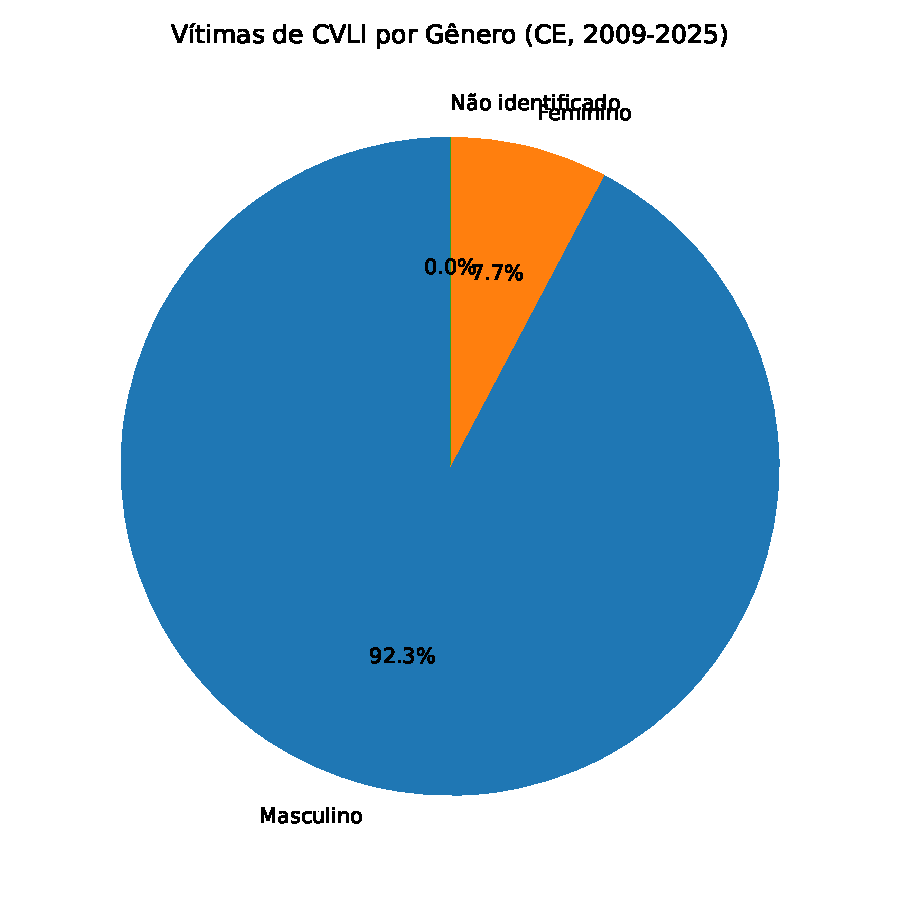
\includegraphics[width=0.6\textwidth]{../figuras/pizza_genero.pdf}
\end{figure}
\fonte{SSPDS/CE (2026). Elaborada pelos autores.}

Observa-se, no Gráfico~\ref{fig:pizza-genero}, que o gênero masculino ocupa quase a totalidade do gráfico de setor (92,3\%), formando uma distribuição extremamente assimétrica. A fatia correspondente ao gênero feminino (7,7\%) é visualmente reduzida, o que evidencia a masculinização expressiva da violência letal no Ceará. Esse padrão é consistente ao longo de todo o período analisado e reflete tanto a maior inserção de homens em dinâmicas de risco (tráfico de drogas, disputas territoriais) quanto fatores socioculturais ligados à resolução violenta de conflitos.

\begin{figure}[H]
\centering
\caption{Distribuição percentual dos CVLI segundo o meio empregado, Ceará, 2009--2025}
\label{fig:pizza-meio}
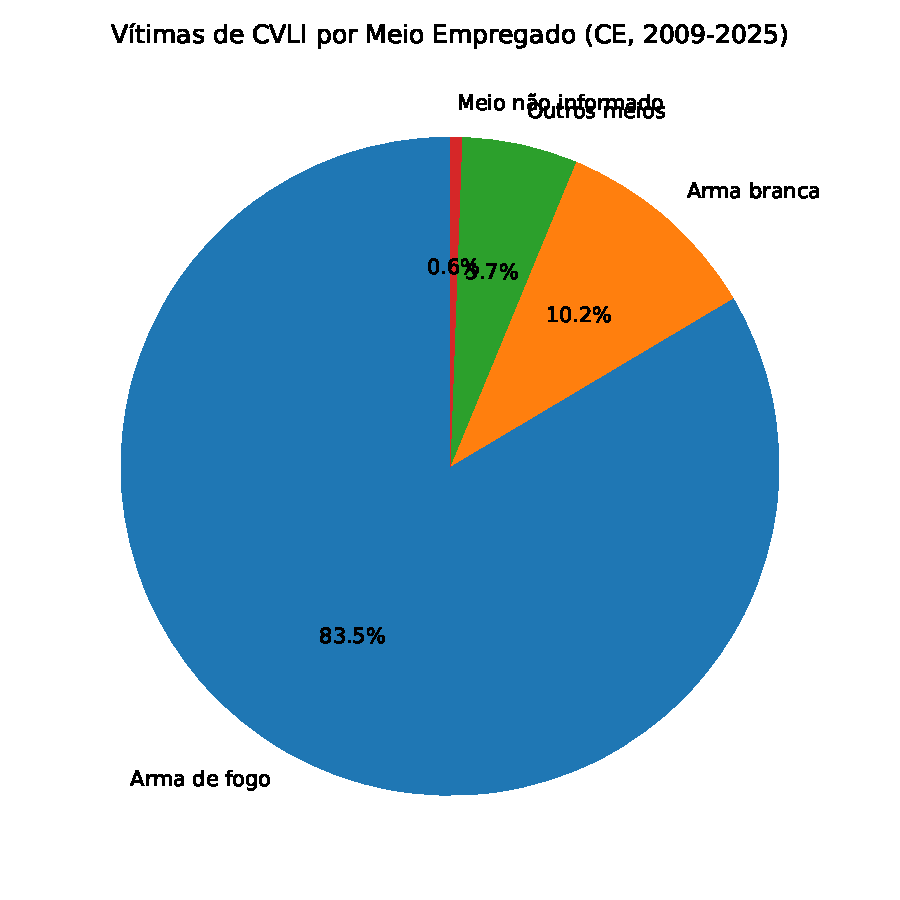
\includegraphics[width=0.6\textwidth]{../figuras/pizza_meio.pdf}
\end{figure}
\fonte{SSPDS/CE (2026). Elaborada pelos autores.}

Conclui-se, a partir do Gráfico~\ref{fig:pizza-meio}, que a arma de fogo domina amplamente o gráfico de setor, ocupando mais de quatro quintos da área (83,5\%). A arma branca (10,2\%) aparece como segunda fatia, seguida de ``Outros meios'' (5,7\%). Essa distribuição evidencia a forte dependência da violência letal cearense em relação às armas de fogo, refletindo a disponibilidade de armamento ilegal no estado e o caráter predominantemente premeditado dos homicídios registrados.


\subsection{Gráficos de barras}


\begin{figure}[H]
\centering
\caption{Frequência dos CVLI por dia da semana, Ceará, 2009--2025}
\label{fig:barra-dia}
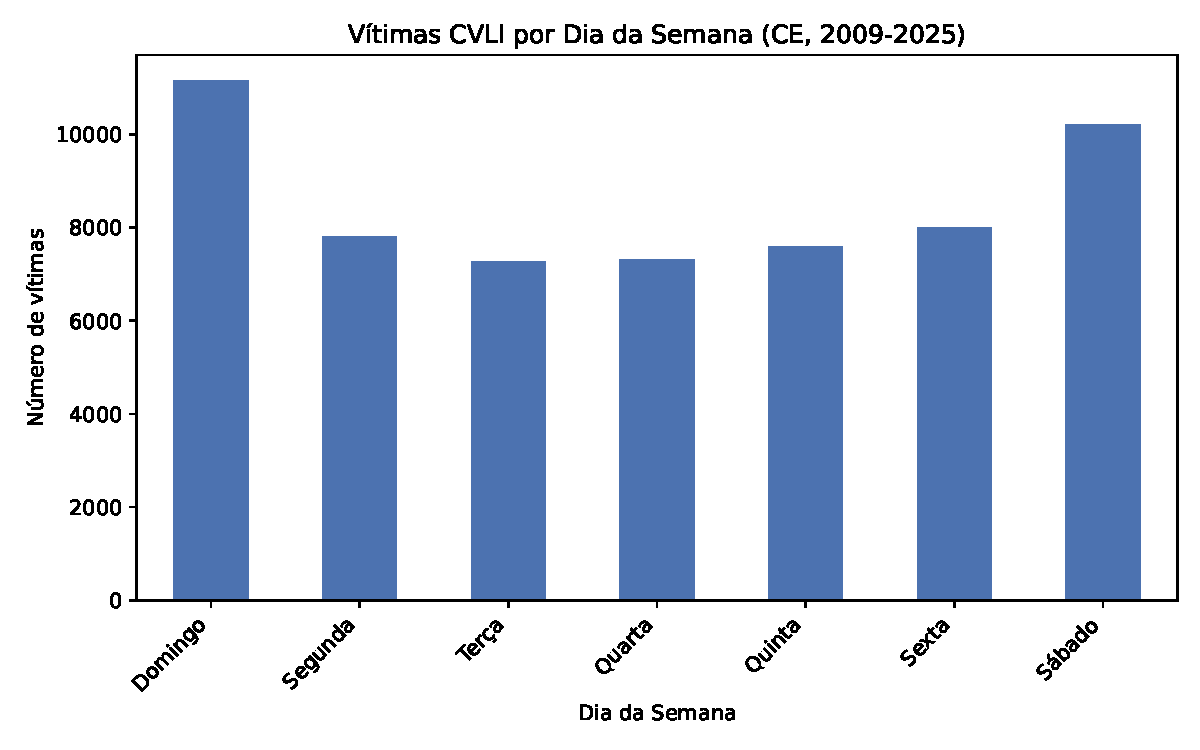
\includegraphics[width=0.8\textwidth]{../figuras/barras_dia.pdf}
\end{figure}
\fonte{SSPDS/CE (2026). Elaborada pelos autores.}

Entende-se, pelo Gráfico~\ref{fig:barra-dia}, que as barras correspondentes a Domingo e Sábado se destacam visivelmente das demais, confirmando a concentração dos CVLI nos finais de semana. Domingo lidera com 11.146 registros, seguido de Sábado com 10.220. Os dias úteis apresentam barras de altura semelhante entre si (entre 7.265 e 7.991), configurando distribuição relativamente uniforme de terça a quinta-feira. Esse padrão é atribuído ao aumento do consumo de álcool, à maior circulação em espaços de lazer noturno e ao efeito do registro formal --- crimes da madrugada de domingo são contabilizados nesse dia.

\begin{figure}[H]
\centering
\caption{Frequência das vítimas de CVLI por nível de escolaridade, Ceará, 2009--2025}
\label{fig:barra-escolaridade}
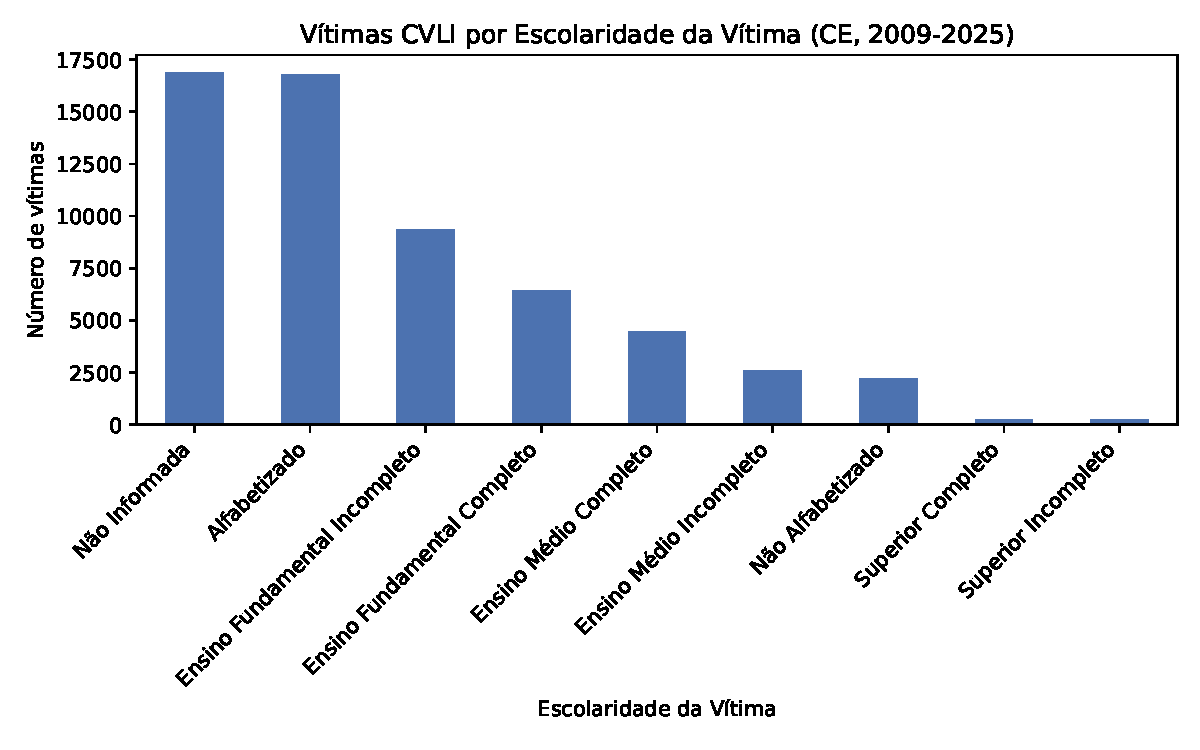
\includegraphics[width=0.8\textwidth]{../figuras/barras_escolaridade.pdf}
\end{figure}
\fonte{SSPDS/CE (2026). Elaborada pelos autores.}

Observa-se, no Gráfico~\ref{fig:barra-escolaridade}, que as barras mais altas correspondem às categorias ``Não Informada'' e ``Alfabetizado'', seguidas de ``Ensino Fundamental Incompleto''. Há uma nítida tendência decrescente à medida que o nível de escolaridade aumenta: as barras correspondentes a ``Superior Incompleto'' e ``Superior Completo'' são praticamente imperceptíveis. Essa distribuição reforça a relação entre vulnerabilidade educacional e risco de vitimização, indicando que a violência letal atinge desproporcionalmente os estratos de menor escolaridade.


\subsection{Gráficos de linha}


\begin{figure}[H]
\centering
\caption{Evolução mensal dos CVLI, Ceará, 2009--2025}
\label{fig:linha-mes}
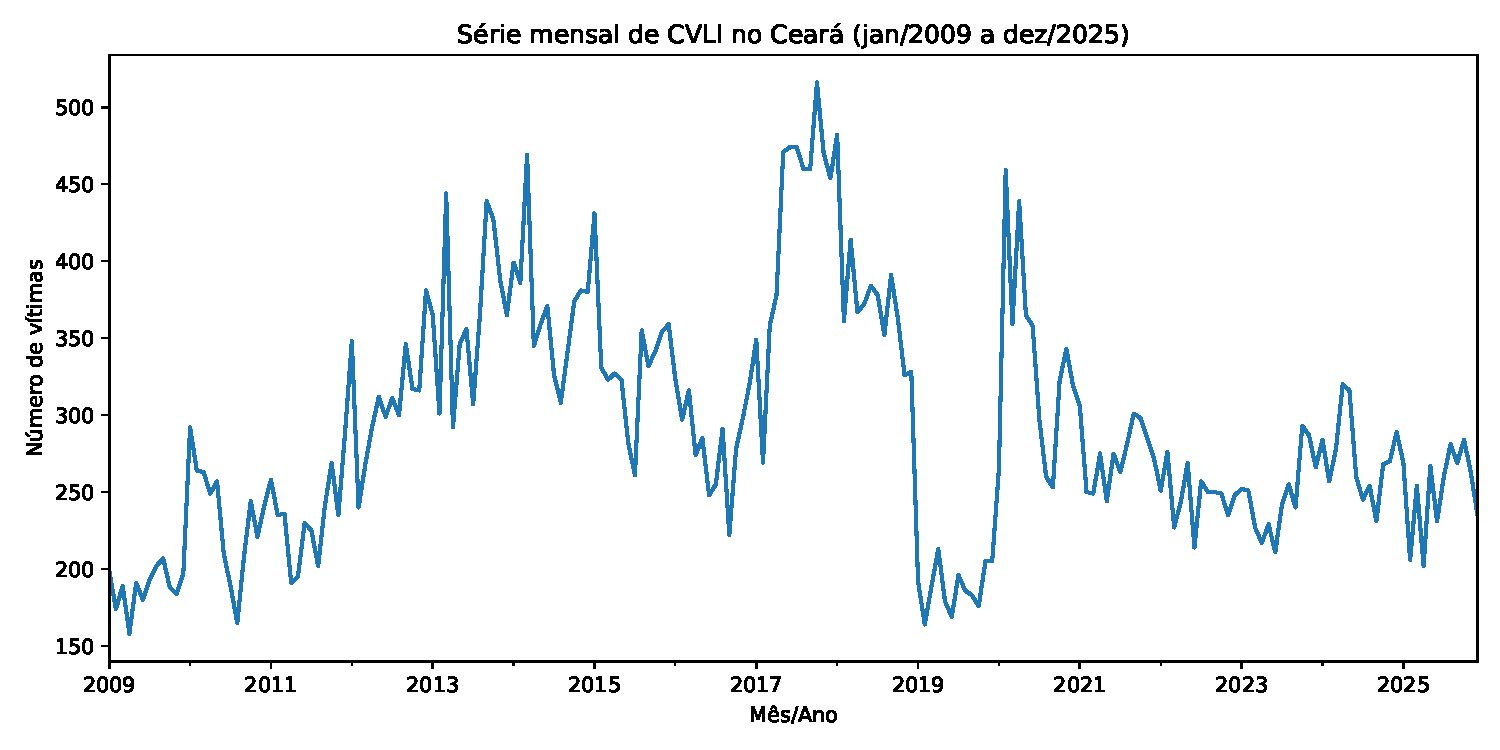
\includegraphics[width=0.9\textwidth]{../figuras/linha_mes.pdf}
\end{figure}
\fonte{SSPDS/CE (2026). Elaborada pelos autores.}

Conclui-se, pelo Gráfico~\ref{fig:linha-mes}, que a série mensal revela sazonalidade marcante, com picos recorrentes no primeiro semestre de cada ano --- especialmente nos meses de janeiro e fevereiro. Esse padrão está associado ao período de festas populares (Carnaval, réveillon), quando o consumo de álcool e a circulação noturna aumentam significativamente. Além disso, a literatura criminológica sugere que grupos criminosos tendem a realizar acertos de contas no início do ano, contribuindo para os picos observados. Visualmente, a série também permite identificar o ciclo de crescimento (2009--2017) e a queda subsequente (2018--2025).

\begin{figure}[H]
\centering
\caption{Evolução anual dos CVLI, Ceará, 2009--2025}
\label{fig:linha-ano}
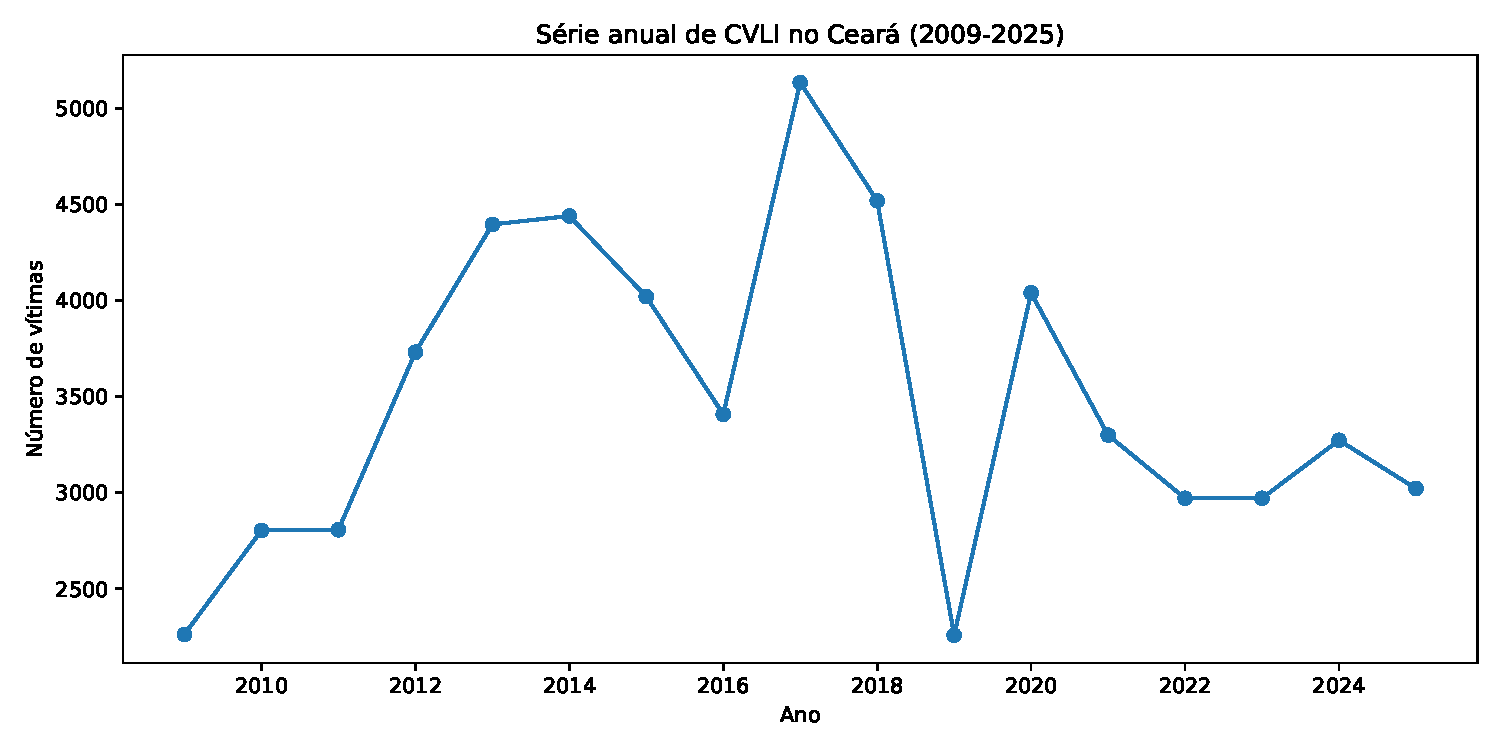
\includegraphics[width=0.9\textwidth]{../figuras/linha_ano.pdf}
\end{figure}
\fonte{SSPDS/CE (2026). Elaborada pelos autores.}

Entende-se, no Gráfico~\ref{fig:linha-ano}, que os CVLI no Ceará apresentam uma trajetória ascendente de 2009 a 2017, quando se atinge o pico da série histórica. A partir de 2018, verifica-se uma inversão da tendência, com queda progressiva que se mantém até 2025. A escalada do período 2009--2017 está associada à expansão das facções criminosas no estado (especialmente a disputa entre CV, PCC e GDE), ao crescimento urbano desordenado nas periferias e à crise econômica de 2015--2016. A queda subsequente reflete a estabilização da disputa territorial entre facções, investimentos em inteligência policial (câmeras, reconhecimento facial), o Programa Ceará Pacífico e, temporariamente, o efeito do isolamento social durante a pandemia de COVID-19 em 2020.

\begin{figure}[H]
\centering
\caption{Distribuição dos CVLI por hora do dia, Ceará, 2009--2025}
\label{fig:linha-hora}
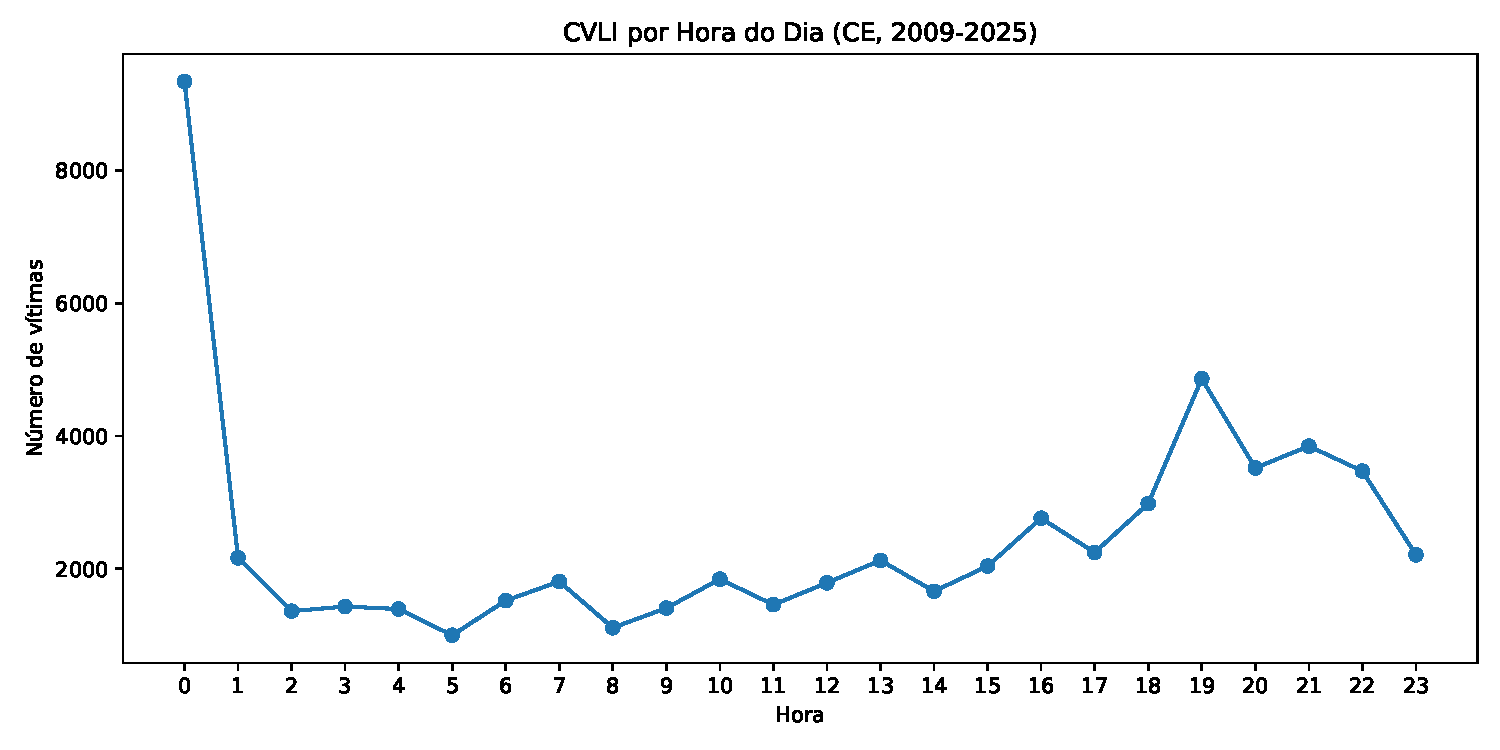
\includegraphics[width=0.9\textwidth]{../figuras/linha_hora.pdf}
\end{figure}
\fonte{SSPDS/CE (2026). Elaborada pelos autores.}

Observa-se, no Gráfico~\ref{fig:linha-hora}, que a distribuição dos CVLI ao longo das 24 horas do dia apresenta formato nitidamente assimétrico, com concentração no período noturno. O pico principal ocorre entre 20h e 23h, com um segundo pico entre 0h e 2h (madrugada). As horas da manhã, entre 6h e 11h, registram os menores valores da série. Esse padrão está diretamente associado ao consumo de álcool e substâncias psicoativas em ambientes de sociabilidade noturna, à redução do efetivo policial nas horas tardias, à dinâmica do tráfico de drogas (mais intenso à noite) e à menor capacidade de resposta do sistema de saúde para atendimento de urgência no período noturno.


\subsection{Medidas de posição e separatrizes --- Idade da vítima}


\begin{table}[H]
\centering
\caption{Medidas de posição e separatrizes da idade das vítimas de CVLI, Ceará, 2009--2025}
\label{tab:posicao}
\begin{tabular}{lr}
\toprule
\textbf{Medida} & \textbf{Valor (anos)} \\
\midrule
Média                       & 29,82 \\
Mediana ($Q_2$)             & 27,0  \\
Moda                        & 20,0  \\
Mínimo                      & 0     \\
Máximo                      & 112   \\
1º Quartil ($Q_1$)          & 21,0  \\
3º Quartil ($Q_3$)          & 36,0  \\
1º Decil ($D_1$)            & 17,0  \\
9º Decil ($D_9$)            & 47,0  \\
Percentil 95 ($P_{95}$)     & 54,0  \\
\bottomrule
\end{tabular}
\end{table}
\fonte{SSPDS/CE (2026). Elaborada pelos autores.}

Conclui-se, com base na Tabela~\ref{tab:posicao}, que as vítimas de CVLI no Ceará são predominantemente jovens. A mediana de 27 anos indica que metade das vítimas tem até essa idade, enquanto a moda de 20 anos revela que essa é a idade mais frequente entre os vitimados. A diferença entre média (29,82) e mediana (27,0) evidencia assimetria positiva na distribuição, puxada por vítimas de idades mais avançadas. O 1º decil ($D_1 = 17$ anos) mostra que 10\% das vítimas são adolescentes, e o intervalo interquartílico ($Q_1 = 21$; $Q_3 = 36$) concentra 50\% das vítimas na faixa de 21 a 36 anos, reforçando a vulnerabilidade da população jovem adulta.


\subsection{Medidas de dispersão --- Idade da vítima}


\begin{table}[H]
\centering
\caption{Medidas de dispersão da idade das vítimas de CVLI, Ceará, 2009--2025}
\label{tab:dispersao}
\begin{tabular}{lr}
\toprule
\textbf{Medida} & \textbf{Valor} \\
\midrule
Amplitude total                     & 112 anos \\
Amplitude interquartílica ($AIQ$)   & 15,0 anos \\
Variância ($s^2$)                   & 148,22 \\
Desvio padrão ($s$)                 & 12,17 anos \\
Coeficiente de variação ($CV$)      & 40,8 \% \\
\bottomrule
\end{tabular}
\end{table}
\fonte{SSPDS/CE (2026). Elaborada pelos autores.}

Entende-se, pela Tabela~\ref{tab:dispersao}, que a variável idade apresenta \textbf{alta dispersão}, com coeficiente de variação de 40,8\% (superior ao limiar de 30\%). A amplitude total de 112 anos é influenciada por valores extremos (\textit{outliers}), como crianças recém-nascidas e idosos acima de 100 anos, cujos registros podem conter erros de digitação. A amplitude interquartílica de 15 anos (de 21 a 36 anos) é mais representativa da variabilidade central e indica que, embora a concentração seja na faixa jovem, há dispersão considerável dentro desse grupo. O desvio padrão de 12,17 anos confirma que as idades se distribuem em uma faixa ampla em torno da média de 29,82 anos.


\subsection{Boxplot --- Idade da vítima}


\begin{figure}[H]
\centering
\caption{Boxplot da idade das vítimas de CVLI, Ceará, 2009--2025}
\label{fig:boxplot}
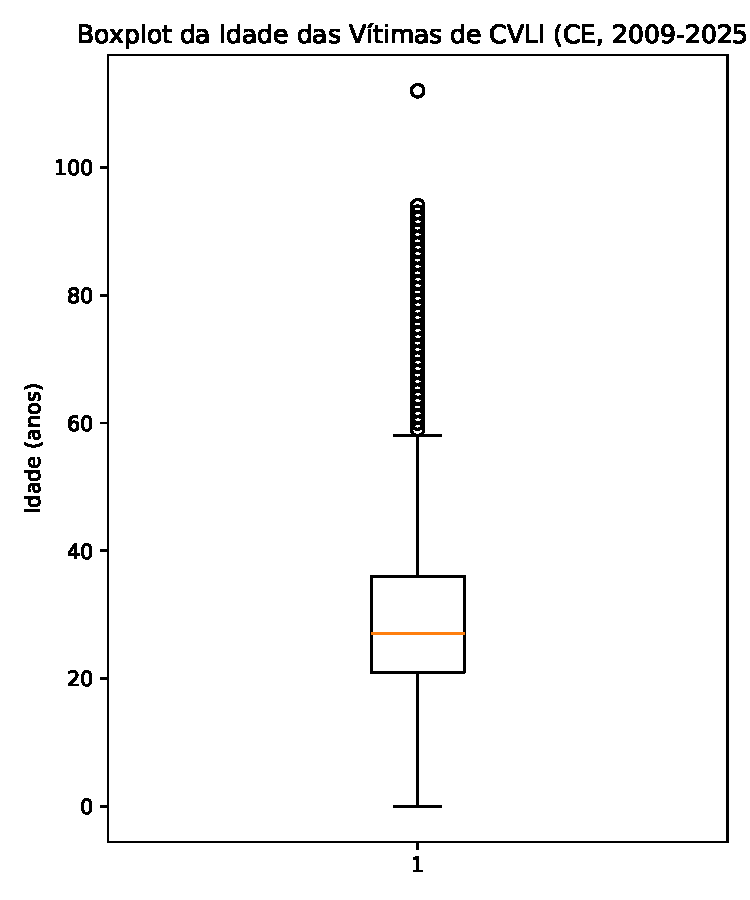
\includegraphics[width=0.6\textwidth]{../figuras/boxplot_idade.pdf}
\end{figure}
\fonte{SSPDS/CE (2026). Elaborado pelos autores.}

Observa-se, no Gráfico~\ref{fig:boxplot}, que a caixa do boxplot situa-se entre 21 e 36 anos (correspondente ao intervalo interquartílico), com a linha mediana posicionada em 27 anos. A caixa é relativamente compacta, confirmando que metade das vítimas concentra-se em uma faixa de apenas 15 anos. As hastes (\textit{whiskers}) estendem-se de forma assimétrica, sendo mais longas no sentido das idades maiores, o que corrobora a assimetria positiva observada nas medidas de posição. A presença de numerosos \textit{outliers} acima da haste superior indica vítimas em faixas etárias mais avançadas, enquanto os \textit{outliers} abaixo da haste inferior correspondem a crianças e adolescentes --- casos frequentemente associados a balas perdidas ou violência intrafamiliar.

\newpage


\section{Conclusão}

A análise descritiva dos registros de CVLI no Estado do Ceará entre 2009 e 2025 permitiu fornecer subsídios estatísticos para a compreensão do cenário da violência letal no estado, atendendo ao objetivo geral proposto.

Quanto à distribuição temporal, conclui-se que os CVLI apresentaram tendência crescente entre 2009 e 2017, atingindo o pico da série nesse último ano, seguida de queda expressiva até 2025. A análise mensal revelou sazonalidade consistente, com maiores registros nos meses de janeiro e fevereiro. Quanto ao horário, a concentração noturna (20h a 2h) é marcante, e os finais de semana (Domingo e Sábado) concentram 36\% de todos os registros.

Em relação ao perfil das vítimas, entende-se que a violência letal no Ceará tem rosto predominantemente masculino (92,3\%), jovem (mediana de 27 anos, moda de 20 anos) e de baixa escolaridade (mais de 44\% com, no máximo, ensino fundamental incompleto entre os registros informados). A variável raça/cor apresentou alto percentual de não preenchimento (77,7\%), limitando conclusões nessa dimensão.

No que se refere ao meio empregado e à natureza dos crimes, verifica-se que a arma de fogo é o instrumento utilizado em 83,5\% dos CVLI, e o homicídio doloso corresponde a 96,7\% das ocorrências, indicando o caráter predominantemente premeditado da violência letal no estado.

Por fim, cabe destacar como limitações da base analisada o alto percentual de campos ``Não Informada'' nas variáveis raça/cor (77,7\%) e escolaridade (28,4\%), que restringem a capacidade analítica e sugerem a necessidade de aprimoramento nos procedimentos de coleta e registro de dados pela SSPDS/CE. Apesar dessas limitações, os resultados apresentados oferecem contribuições relevantes para o direcionamento de políticas públicas de segurança, especialmente no que diz respeito à proteção de jovens do sexo masculino em situação de vulnerabilidade socioeconômica, ao reforço da vigilância policial nos finais de semana e no período noturno, e ao combate ao tráfico de armas de fogo.

\newpage


\section*{Referências Bibliográficas}
\addcontentsline{toc}{section}{Referências Bibliográficas}

\begin{description}
\item CEARÁ. Secretaria da Segurança Pública e Defesa Social. \textbf{Estatísticas: dados detalhados --- indicadores detalhados 2009 a 2025}. Fortaleza, 2026. Disponível em: \url{https://www.ce.gov.br/sspds/estatisticas/dados-detalhados/}. Acesso em: 07 set. 2026.

\item BUSSAB, W. O.; MORETTIN, P. A. \textbf{Estatística básica}. 9. ed. São Paulo: Saraiva, 2017.

\item MCKINNEY, W. \textbf{Python for data analysis}. 3. ed. Sebastopol: O'Reilly Media, 2022.

\item FÓRUM BRASILEIRO DE SEGURANÇA PÚBLICA. \textbf{Anuário Brasileiro de Segurança Pública 2023}. São Paulo: FBSP, 2023.

\item IPEA. \textbf{Atlas da Violência 2023}. Rio de Janeiro: Instituto de Pesquisa Econômica Aplicada, 2023.
\end{description}

\newpage


\appendix
\section{Rotina Computacional em Python}
\label{ap:codigo}

\begin{lstlisting}[style=python,caption={Trecho da rotina de leitura e análise descritiva},captionpos=b]
import pandas as pd
import numpy as np
import matplotlib.pyplot as plt

# Leitura da base
df = pd.read_excel("cvli_ce_2009_2025.xlsx")

# Frequencia simples e relativa
tab = df["MEIO EMPREGADO"].value_counts().to_frame("f")
tab["%"] = (tab["f"] / tab["f"].sum() * 100).round(1)
print(tab)

# Medidas de posicao e dispersao da idade
idade = pd.to_numeric(df["IDADE"], errors="coerce").dropna()
print(idade.describe())
print("Moda:", idade.mode()[0])
print("CV:", round(idade.std() / idade.mean() * 100, 1), "%")
\end{lstlisting}

\end{document}